\begin{frame}{Working with Data}
    \framesubtitle{The Problem with Full-Batch Updates}
    \begin{itemize}
        \item In standard (or "batch") gradient descent, we compute the gradient by averaging over the \bhighlight{entire training dataset} for a single update step.
        \[ \nabla_{w}E(W) = \frac{1}{N} \sum_{n=1}^{N} \nabla_{w}\text{loss}(f(x^{(n)}; W), y^{(n)}) \]
        \item \textbf{The Problem:} For modern datasets with millions of examples, this is extremely slow. We have to process all data just to make one small step.
    \end{itemize}
    \begin{figure}
        \centering
        % Source: Optimization II.pdf, Page: 11
        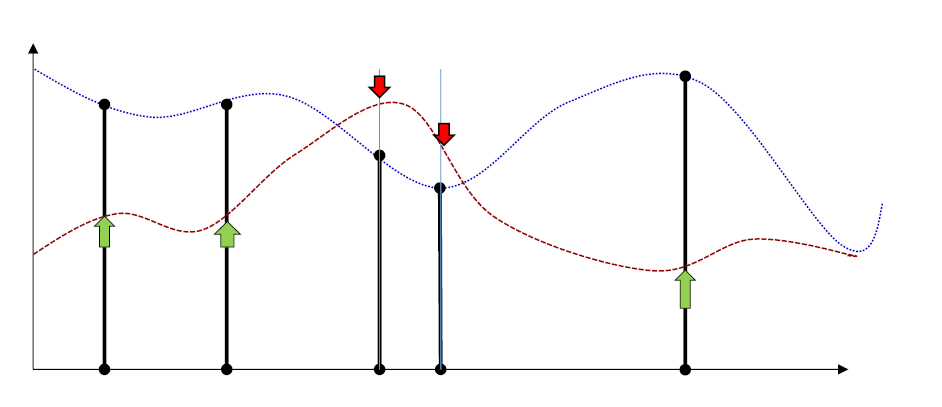
\includegraphics[width=0.7\linewidth]{images/full_batch_idea.png}
        \caption{In batch gradient descent, the algorithm tries to adjust the model based on all training points simultaneously.}
    \end{figure}
\end{frame}

\begin{frame}{Stochastic Gradient Descent (SGD)}
    \framesubtitle{Updating One Sample at a Time}
    \begin{itemize}
        \item The other extreme is \bhighlight{Stochastic Gradient Descent (SGD)}, where we update the weights after seeing \emph{only one} training example at a time.
        \item This makes each update much faster, allowing us to make many more updates in the same amount of time.
    \end{itemize}
    \begin{figure}
        \centering
        % Source: Optimization II.pdf, Page: 15
        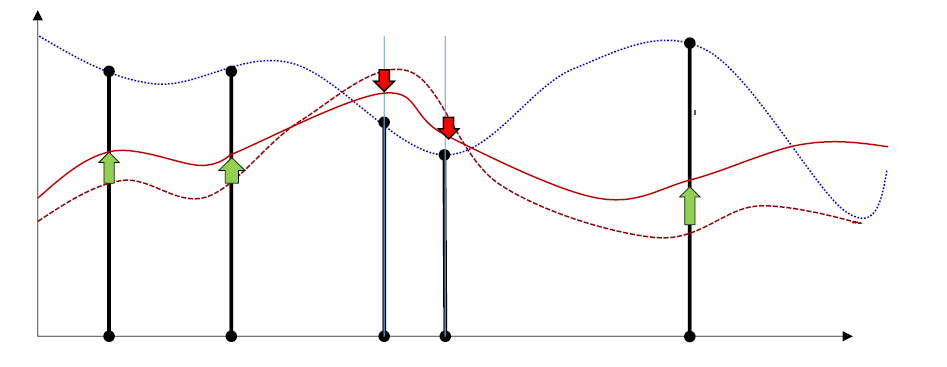
\includegraphics[width=0.7\linewidth]{images/sgd_step_1.png}
        \caption{With SGD, the function is first adjusted for a single, random training point...}
    \end{figure}
\end{frame}

\begin{frame}{Stochastic Gradient Descent (SGD)}
    \framesubtitle{Iterating Through Samples}
    \begin{figure}
        \centering
        % Source: Optimization II.pdf, Page: 16
        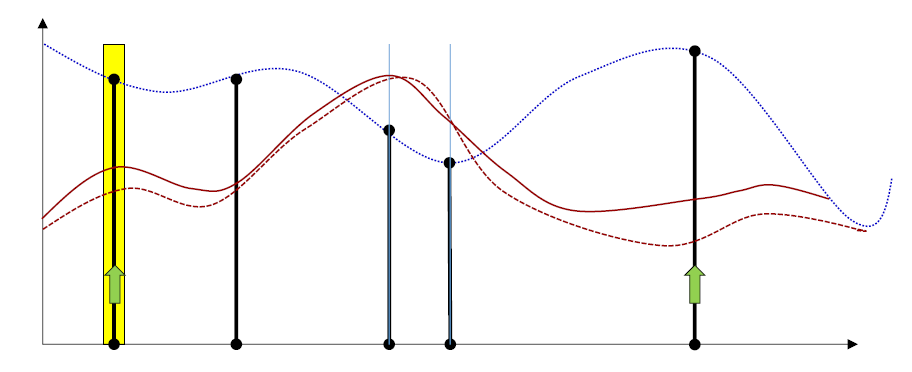
\includegraphics[width=0.7\linewidth]{images/sgd_step_2.png}
        \caption{...then it is adjusted for the next random point...}
    \end{figure}
\end{frame}

\begin{frame}{Stochastic Gradient Descent (SGD)}
    \framesubtitle{Completing an Epoch}
    \begin{figure}
        \centering
        % Source: Optimization II.pdf, Page: 17
        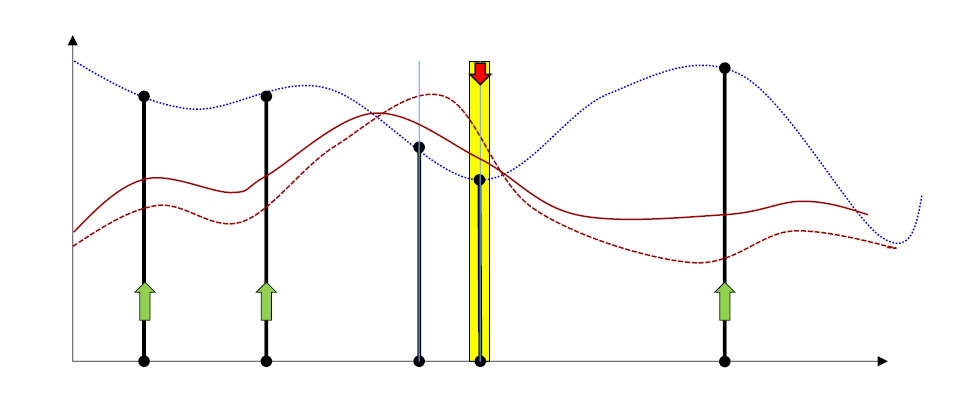
\includegraphics[width=0.7\linewidth]{images/sgd_step_3.png}
        \caption{...and so on. After passing through all points once (an epoch), the entire function has been adjusted.}
    \end{figure}
\end{frame}

\begin{frame}{Stochastic Gradient Descent (SGD)}
    \framesubtitle{The Algorithm and Key Concepts}
    \begin{itemize}
        \item \textbf{The Update Rule:} For a single sample $(x^{(n)}, y^{(n)})$:
        \[ w^{t+1} = w^{t} - \eta \nabla_{w}\text{loss}(f(x^{(n)}; W), y^{(n)}) \]
        \item \textbf{Epoch:} A single full pass through the entire training dataset is called an \bhighlight{epoch}. In one epoch of SGD, we make N weight updates.
        \item \textbf{Crucial Requirement:} For SGD to work correctly, the training data must be \bhighlight{shuffled} at the beginning of every epoch. This randomness is essential for good convergence.
    \end{itemize}
\end{frame}

\begin{frame}{Stochastic Gradient Descent (SGD)}
    \framesubtitle{The "Stochastic" Nature}
    \begin{itemize}
        \item The gradient from a single sample is a "noisy" but \bhighlight{unbiased estimate} of the true gradient over the full dataset.
        \item This high variance means the path to the minimum is erratic and jittery.
    \end{itemize}
    \begin{figure}
        \centering
        % Source: Optimization II.pdf, Page: 47 (zoomed on SGD path)
        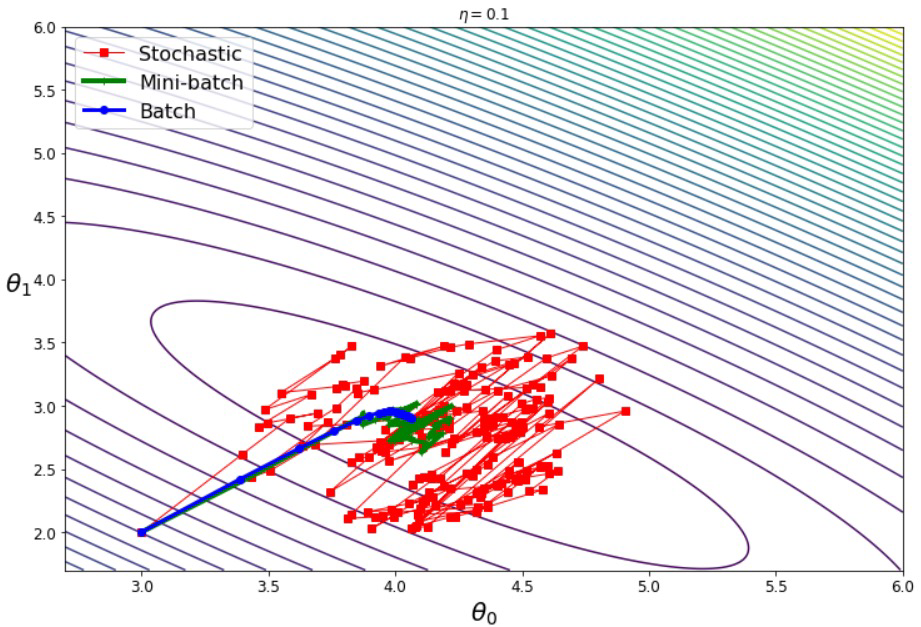
\includegraphics[width=0.6\linewidth]{images/sgd_pathj.png}
        \caption{The path of SGD is very noisy due to the high variance of single-sample gradients.}
    \end{figure}
\end{frame}

\begin{frame}{Mini-Batch Gradient Descent}
    \framesubtitle{The Best of Both Worlds}
    \begin{itemize}
        \item \bhighlight{Mini-Batch Gradient Descent} is the standard method used in practice. It's a compromise between the full-batch and SGD approaches.
        \item We compute the gradient on a small, random subset of the data called a \bhighlight{mini-batch}.
    \end{itemize}
    \begin{figure}
        \centering
        % Source: Optimization II.pdf, Page: 24
        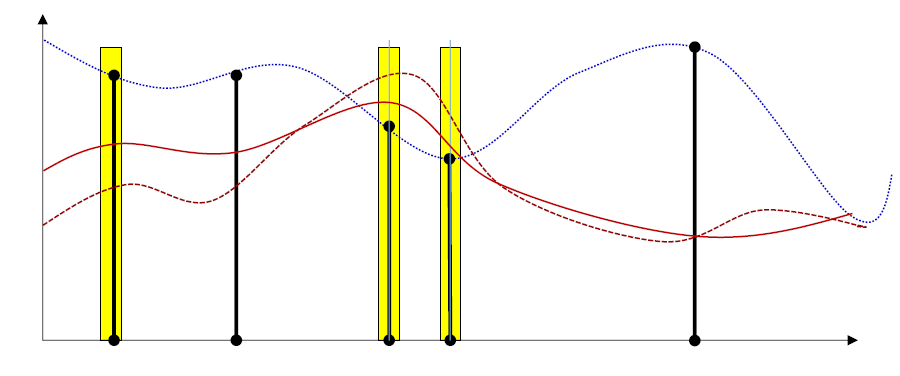
\includegraphics[width=0.7\linewidth]{images/minibatch_idea.png}
        \caption{In Mini-Batch GD, we update the model based on a small, random subset of the data.}
    \end{figure}
\end{frame}

\begin{frame}{Mini-Batch Gradient Descent}
    \framesubtitle{Advantages}
    \begin{itemize}
        \item \textbf{Efficiency:} It allows us to take advantage of the massive parallelization capabilities of GPUs. Matrix operations on a mini-batch are much more efficient than processing samples one by one.
        \item \textbf{Stability:} By averaging gradients over a small batch, we reduce the variance of the updates, leading to a more stable convergence than pure SGD.
    \end{itemize}
\end{frame}

\begin{frame}{Comparing the Update Strategies}
    \framesubtitle{A Visual Guide}
    \begin{figure}
        \centering
        % Source: Optimization II.pdf, Page: 47
        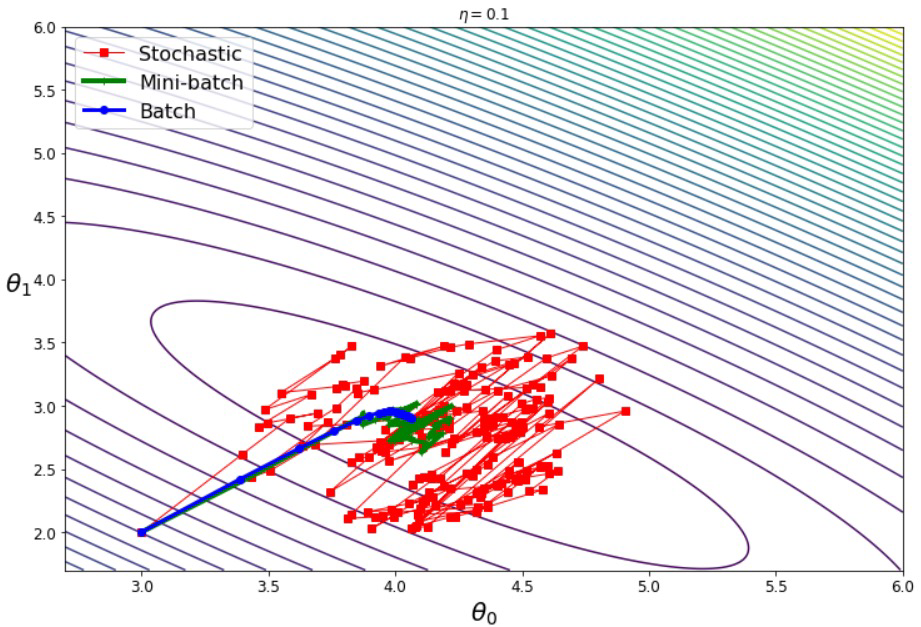
\includegraphics[width=0.9\linewidth]{images/optimizer_paths.png}
        \caption{
            \textbf{Batch (Blue):} Takes a smooth, direct path but each step is very slow.
            \textbf{Stochastic (Red):} Very noisy and erratic path, but takes many fast steps.
            \textbf{Mini-Batch (Green):} A good balance, reducing noise while still being computationally efficient.
        }
    \end{figure}
\end{frame}

\begin{frame}{Choosing the Mini-Batch Size}
    \framesubtitle{A Practical Guideline}
    \begin{itemize}
        \item The mini-batch size is a hyperparameter that needs to be chosen.
        \item If the training set is very small (e.g., < 2000 examples), you can often use full-batch gradient descent.
        \item For larger datasets, typical mini-batch sizes are powers of 2, such as \bhighlight{32, 64, 128, 256, 512}.
        \item A key constraint is that the mini-batch of data and the resulting gradients must fit into your GPU's memory.
    \end{itemize}
\end{frame}